\normaltrue \difficilefalse \tdifficilefalse
\correctionfalse

%\UPSTIidClasse{11} % 11 sup, 12 spé
%\newcommand{\UPSTIidClasse}{11}

\exer{Calcul de FTBO$\star$ \label{B2:07:505}}
\setcounter{numques}{0}
\UPSTIcompetence[2]{B2-07}
\index{Compétence B2-07}
\index{Schéma-blocs}
\index{FTBO}

\ifcorrection
\else
\textbf{Pas de corrigé pour cet exercice.}
\fi


\question{Déterminer la FTBO dans la cas suivant.}
\ifprof 
\else
\begin{center}
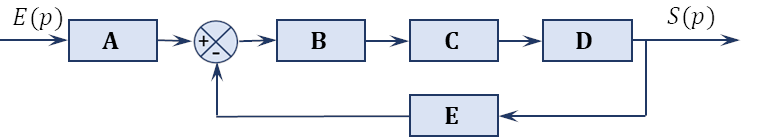
\includegraphics[width=.9\linewidth]{505_01}
\end{center}
\fi
 
\question{Déterminer la FTBO dans la cas suivant.}
\ifprof 
\else
\begin{center}
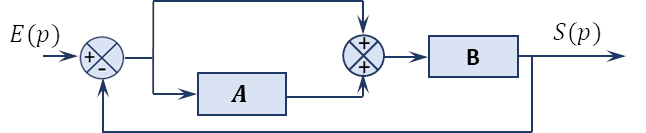
\includegraphics[width=.9\linewidth]{505_02}
\end{center}
\fi

\question{Déterminer la FTBO dans la cas suivant.}
\ifprof 
\else
\begin{center}
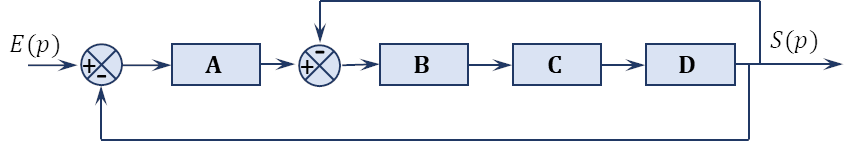
\includegraphics[width=.9\linewidth]{505_03}
\end{center}
\fi

\question{Déterminer la FTBO dans la cas suivant.}
\ifprof 
\else
\begin{center}
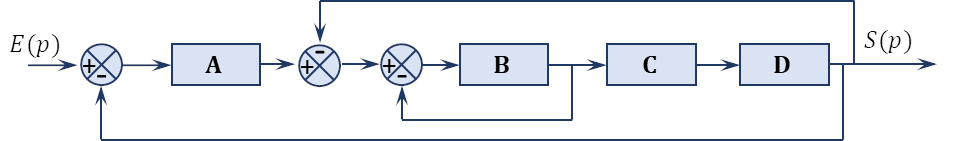
\includegraphics[width=.9\linewidth]{505_04}
\end{center}
\fi



%\question{Réaliser le schéma-blocs.}
%\ifprof
%\begin{figure}[H]
%\centering
%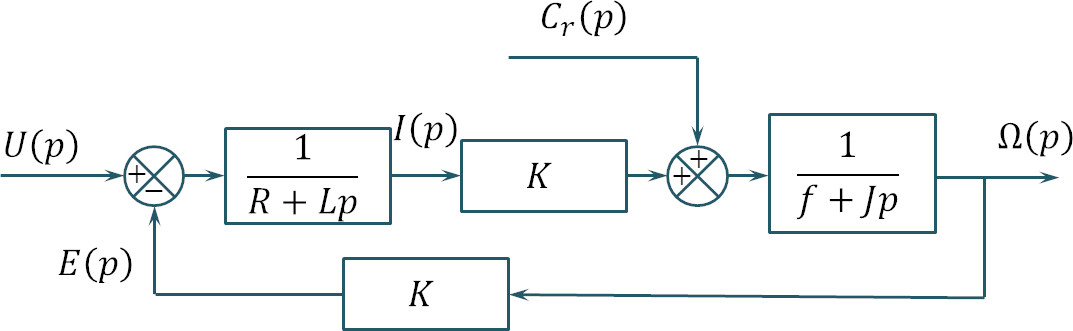
\includegraphics[width=\linewidth]{51_01_c}
%%\caption{Évolution du couple utile en fonction de la vitesse de rotation pour des
%%fréquences de commande de \SI{90}{Hz} à \SI{110}{Hz}. \label{fig_50_04}}
%\end{figure}
%\else
%\fi


 

\ifprof
\else
\begin{flushright}
\footnotesize{Corrigé  voir \ref{B2:07:505}.}
\end{flushright}%
\fi